\section{Alfadian Owen (1174091)}
\subsection{Buku}
Rp.100.000(Lunas)
\subsection{Data Geospasial}
\begin{itemize}
	\item Geospatial data atau Spatial data adalah informasi yang memiliki aspek geografis. dengan kata lain, catatan dalam jenis informasi ini memiliki koordinat, alamat, kota, kode pos.
	\item Tipe dari data geospalsial
	\begin{enumerate}

	\item Vector terdiri dari sudut dan jalur. terdapat tiga tipe dasar data vektor yaitu titik, garis, poligon (area). setiap titik, garis, dan poligon memiliki kerangka referensi spasial seperti lintang dan bujur. titik vektor hanyalah kooridinat XY. garis vektor menghubungkan setiap titik atau simpul dengan jalur dalam urutan tertentu. poligon bergabung dengan satu set simpul
	
	\item Data raster terdiri dari pixel atau grid cells. Biasanya, mereka berbentuk persegi dan berjarak secara teratur. Tapi raster juga bisa persegi panjang. Raster mengaitkan nilai ke setiap piksel. Raster berkelanjutan memiliki nilai yang berubah secara bertahap seperti ketinggian atau suhu. Tetapi raster diskrit mengatur setiap piksel ke kelas tertentu.
	\item Geographic Database. Tujuan dari basis data geografis adalah untuk menampung vektor dan raster. Database menyimpan data geografis sebagai kumpulan data / informasi yang terstruktur.
	\item Web Files. Geodata memiliki jenis penyimpanan dan aksesnya sendiri. seperti GeoJSON, GeoRSS, dan Web Mapping Services (WMS) dibangun untuk melayani dan menampilkan fitur geografis melalui internet
	\item Data multi-temporal melampirkan komponen waktu ke informasi. tetapi geodata multi-temporal tidak hanya memiliki komponen waktu, tetapi juga komponen geografis


	\end{enumerate}
\end{itemize}

\subsection{Link}
https://youtu.be/nm1Zn3VcI2U
\subsection{Plagiarism}'\begin{figure}[H]
	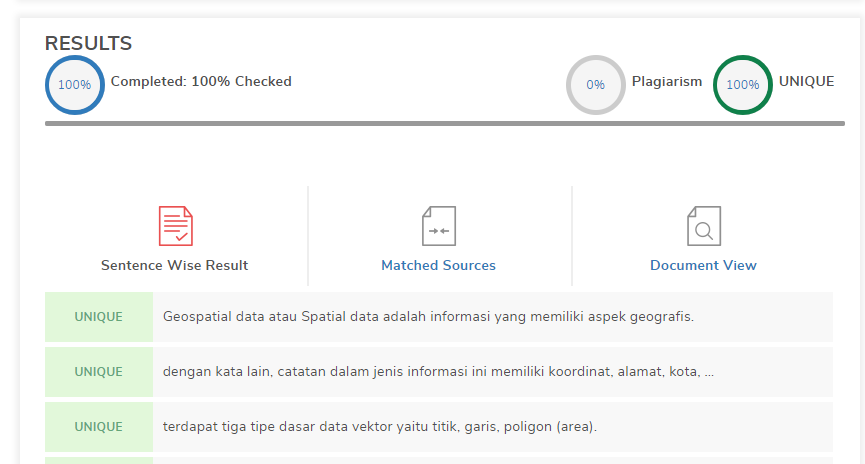
\includegraphics[width=8cm]{figures/Tugas1/1174091/plagiarisme.png}
	\centering
	\caption{Plagiarisme.}
\end{figure}	

\subsection{Cara Penggunaan}
\subsubsection{Gambar}

\hfill\break

Contoh Gambar
\begin{figure}[H]
	
\includegraphics[width=4cm]{figures/himatif.png}
	\centering
	\caption{Contoh gambar.}
\end{figure}

\subsubsection{List}
\begin{enumerate}
	\item Satu
	\item Dua
\end{enumerate}

\begin{itemize}
	\item Satu
	\item Dua
\end{itemize}

